\chapter{Sylviculture et qualité du bois}

\begin{abstract}
	Dans ce chapitre nous définissons d'abord le concept de qualité du bois. Nous faisons ensuite un bref survol des différents travaux sylvicoles à la disposition des forestier pour cultiver et régénérer la forêt. Finalement, les bases permettant d'estimer les effets des traitements sylvicoles sur la qualité du bois sont présentées.
\end{abstract}

\minitoc

\section{Le concept de qualité du bois}

On peut définir la qualité du bois comme une série d’attributs qui rendent le bois approprié pour des usages donnés. \textbf{Le concept de \og qualité \fg du bois n'est pas absolu, mais relatif à un produit donné}.

Quelques caractéristiques du bois sont désirables pour certains usages mais indésirables pour d’autres. Par exemple, pour le bois de charpente, on recherche du bois rigide, présentant une bonne résistance mécanique associée à des nœuds de petite taille et à un fil droit (\textit{Pseudotsuga menziesii; Picea spp.}). Pour la sculpture, on recherche des bois stables, tendres et de masse volumique homogène (\textit{Chamaecyparis nootkatensis; Tilia americana}). Pour le revêtement des planchers et le meubles, on recherche des bois de dureté élevée et de couleur appréciée des consommateurs (\textit{Acer spp., Quercus spp., Betula alleghaniensis, Fraxinus americana}…). Pour la fabrication du papier on recherche du bois possédant des fibres longues à parois cellulaires minces, l’affaissement des parois cellulaires donnant un papier moins poreux mais plus résistant mécaniquement.

\section{Les bases de la sylviculture}
\subsection{Définition de la sylviculture}
On peut définir la sylviculture comme la science qui vise à cultiver la forêt pour en retirer le maximum de biens et de services pour la collectivité. Elle consiste en un ensemble de techniques visant à modeler les caractéristiques des peuplements forestiers de manière à ce qu'ils répondent mieux aux objectifs d'aménagement qu'on leur a fixés. Pour ce faire, elle utilise divers moyens, dont la récolte, la régénération et les différents soin d'éducation. 

\subsection{Procédés de régénération de la forêt}
Les \og précédés de régénération \fg font référence à la coupe forestière qui, d'un point de vue sylvicole, servent à régénérer la forêt. Évidemment, dans le contexte plus large de l'aménagement forestier, on les pratique dans le but d'approvisionner une ou des usines de transformation.

\subsubsection{La coupe totale}\label{cprs}

Dans la méthode par coupe totale, la régénération du peuplement est prévue à la toute fin de la révolution, après l'abattage en coupe unique de tous les arbres contenus dans la superficie à régénérer (Figure \ref{fig:CPRS}). L'expression \og coupe avec protection de la régénération (CPRS) a été popularisée au Québec pour désigner une approche qui consiste à protéger la régénération préexistante lors des opérations de récolte. L'approche consiste à utiliser un système de sentiers dans lesquels la machinerie circule. Ainsi, seule une partie de la régénération préétablie (et du sol) est perturbée par les opérations.\\

\begin{figure}[!h]
\centering
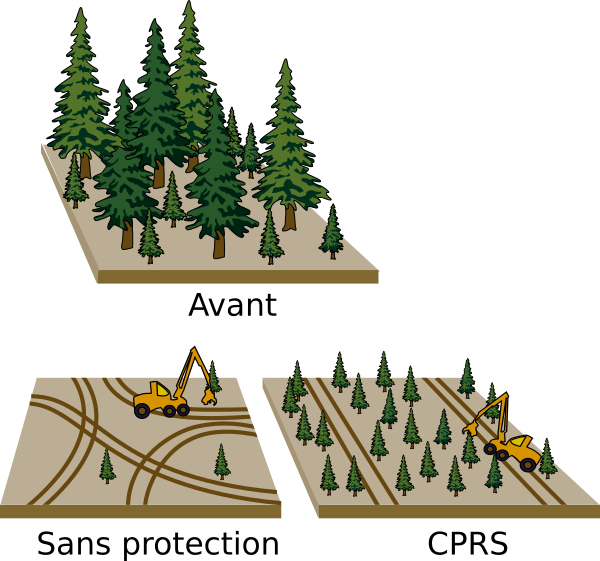
\includegraphics[width=0.7\linewidth]{./img/ch8_CPRS}
\caption{Procédé de régénération par coupe totale. Le système de sentiers de récolte permet de protéger la régénération. CPRS = coupe avec protection de la régénération et des sols}
\label{fig:CPRS}
\end{figure}

Évidemment, dans le cas de la coupe totale, l'ensemble des tiges de diamètre marchand sont envoyées à l'usine de transformation en une seule étape. La qualité des approvisionnements dépend donc des caractéristiques du peuplement au moment de la coupe.

\subsubsection{L'établissement de la régénération par coupe progressive}\label{cprog}

La caractéristique la plus fondamentale de la régénération par coupes progressives réside dans le fait que l'établissement du nouveau peuplement débute \textbf{avant la fin de la révolution du peuplement en place}. Ainsi, les semis installés profitent de la protection d'un couvert forestier pendant quelques années. Ce procédé conduit à la récolte complète du peuplement à travers une série de coupes partielles qui surviennent en fin de révolution (Figure \ref{fig:cprog}). Le principe du procédé veut que le peuplement soit ouvert de façon progressive pour favoriser l'établissement et le développement des jeunes semis, tout en donnant à ceux-ci une protection suffisante en présence de conditions adverses. Dans ce procédé, on considère deux types de coupes: la coupe d'ensemencement et la coupe finale.

\begin{description}
\item[La coupe d'ensemencement] La coupe d'ensemencement, tout en favorisant aussi une bonne production de graines, vise principalement à obtenir un éclairement au sol propice à la germination et à l'installation des espèces désirables. On favorise le plus possible la rétention des arbres des essences recherchées (qui servent d'apport de semences) aux dépens des autres.\\ 

Ainsi, le choix des arbres lors de cette coupe dite \og partielle \fg aura une influence sur la qualité des approvisionnements. Ceux-ci seront possiblement constitués d'une proportion plus élevée d'essences peu désirées par rapport à la coupe finale. Comme il y a un délai de quelques années entre les deux coupes, la taille moyenne des arbres sera aussi plus faible que lors de la coupe finale. 

\item[La coupe finale] : C'est la dernière coupe qui élimine tous les grands arbres encore en place. Elle vise à donner la pleine lumière au nouveau peuplement. Il s'agit en fait d'une \hyperref[cprs]{CPRS}.
\end{description}

\begin{figure}[!h]
\centering
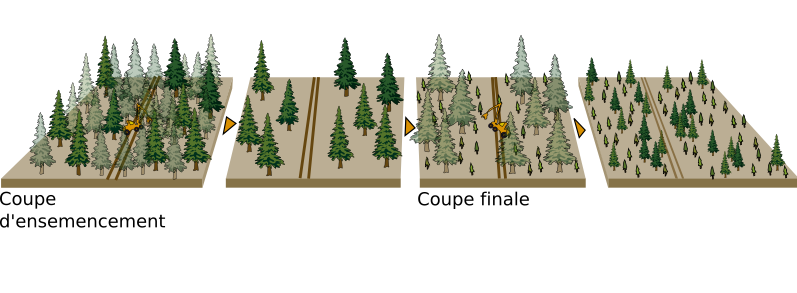
\includegraphics[width=1\linewidth]{./img/ch8_CPI}
\caption{ Procédé de régénération par coupe progressive}
\label{fig:cprog}
\end{figure}


\subsubsection{La coupe de jardinage}

Certains peuplement forestiers contiennent des arbres de tous les âges, et donc de toutes les tailles. C'est couvent le cas dans nos forêts feuillues tempérées. Dans ce contexte, la coupe de jardinage permet d'assurer la régénération, la récolte et l'éducation du peuplement dans une seule intervention. Elle vise à établir ou maintenir une structure dite \og inéquienne \fg dans le peuplement.\\

En principe, les arbres sont récoltés à mesure qu'ils arrivent à maturité, ce qui crée une trouée dans le couvert. Ils seront remplacés par des semis déjà à leur place au moment de la coupe ou par une nouvelle cohorte de semis qui s'établissent et se développent en profitant de nouvelles conditions plus favorables (nouvel apport de lumière au sol).\\

Une partie seulement du peuplement est enlevée, de sorte qu'on peut le perpétuer indéfiniment et, s'il est appliqué selon les règles de l'art, extraire périodiquement des tiges de haute qualité et de dimension désirées. Les règles de l'art dictent que ce sont les arbres de faible vigueur qui devraient être récoltés en priorité, puisque ceux-ci sont susceptibles d'être morts lors de la prochaine intervention. En procédant à l'inverse, c'est-à-dire en choisissant les tiges de meilleure qualité, souvent vigoureuses, on procède à un écrémage progressif de la forêt. La ligne est donc mince entre la nécessité d'approvisionner une usine en bois de qualité dans l'immédiat et de maintenir le capital forestier nécessaire à la production de tiges de qualité dans l'avenir.\\
	
Dans une \textbf{coupe de jardinage} théoriquement, chaque groupe de structure équienne composant le peuplement de structure inéquienne occupe la place d'un arbre enlevé à maturité (Figure \ref{fig:jardinage_pied}). Immédiatement après la coupe, quelques milliers de semis sont installés dans la trouée laissée par un seul arbre récolté. Au stade du gaulis, quelques centaines d'individus demeurent et leur nombre diminuera jusqu'à quelques dizaines de perches par la suite. Lors de l'intervention, la récolte devrait théoriquement s'effectuer dans chacun des \hyperref[developpement]{stades de développement} du peuplement (Figure~\ref{fig:jardinage}).
	
	\begin{figure}[!h]
		\centering
		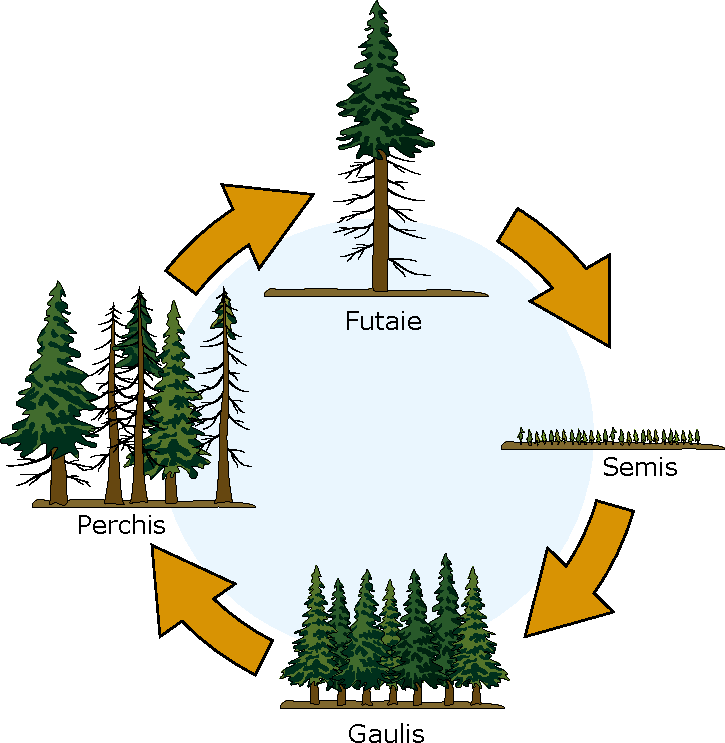
\includegraphics[width=0.6\linewidth]{./img/ch8_jardinage_pied}
		\caption{Théoriquement, dans le jardinage par pied d'arbre, chaque groupe de structure équienne composant le peuplement de structure inéquienne occupe la place d'un arbre enlevé à maturité}
		\label{fig:jardinage_pied}
	\end{figure}
	
	\begin{figure}[!h]
		\centering
		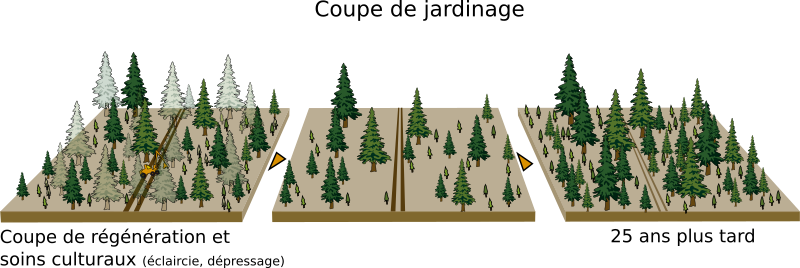
\includegraphics[width=1\linewidth]{./img/ch8_jardinage}
		\caption{Procédé de régénération par coupe de jardinage par pied d'arbre}
		\label{fig:jardinage}
	\end{figure}	


Au Québec, on peut dire que le potentiel de ce procédé de régénération a été démontré à une échelle expérimentale, mais que la possibilité de l'appliquer avec succès à l'échelle industrielle reste à démontrer. C'est face à ce constat que la méthode MSCR qui guide l'évaluation de la vigueur des arbres a été développée.\\

Le guide contient une grille d'évolution des défauts des arbres permettant d'évaluer la priorité de récolte. Celle-ci est basée sur plusieurs éléments qui doivent être vérifiés par le marteleur. L'identification de l'essence, du défaut externe le plus important, de l'endroit où siège ce défaut ainsi que l'origine de celui-ci constitue la première étape à franchir pour identifier la classe de vigueur actuelle de l'arbre. Cette information permet alors d'identifier la priorité de récolte des tiges.\\

Il existe 4 niveaux de vigueur qui se définissent ainsi \citep{boulet2007defauts} :

\begin{itemize}
	\item Priorité 1 - \textbf{M, mourir} : Tige très défectueuse, qui risque de se renverser, de se rompre ou de mourir sur pied avant la prochaine rotation. Arbre moribond ou en perdition.
	\item Priorité 2 - \textbf{S, survie} : Tige défectueuse en perdition dont le volume de bois risque de diminuer en raison de la carie, mais dont la survie n'est pas compromise avant la prochaine rotation. Arbre en décroissance.
	\item Priorité 3 - \textbf{C, conservé} : Tige peu défectueuse à conserver, dont le volume de bois marchand ne risque pas de se dégrader avant la prochaine rotation. Arbre en croissance.
	\item Priorité 4 – \textbf{R, réserve }: Tige saine en réserve idéalement dégagée pour croître librement, qui constitue le capital forestier de premier choix. Arbre d'avenir en réserve.	
\end{itemize}

Notez que cette classification ne tient pas directement compte de la qualité du bois. Elle cherche seulement à évaluer la probabilité qu'une tige soit vivante lors du prochain passage dans le peuplement (la prochaine coupe prévue dans 20 ou 25 ans dans le cas du jardinage). Une fois cette probabilité établie, on doit récolter les tiges les plus susceptibles de mourir rapidement. Afin d'assurer la rentabilité du traitement sylvicole, il importe de récolter en priorité les arbres non vigoureux ayant conservé une qualité suffisante pour le sciage.\\

\subsubsection{Classes de qualité (A-B-C-D)}
Au Québec, la détermination de classes de qualité sur les arbres debout s'applique surtout au feuillus puisque la \og qualité \fg des tiges pour le sciage et le déroulage (qui mènent à des produits à haute valeur ajoutée) diffère grandement entre les individus, contrairement aux résineux. La classification est inspirée des normes de classification des billes (bois abattus). Ces dernières servent au calcul des droits de coupe que doivent verser les compagnies œuvrant sur terres publiques \citep{MRNF2009taux}. Chez les résineux du groupe SEPM (sapin, épinettes, pin gris, mélèze), il n'existait jusqu'à tout récemment qu'une seule classe de qualité. Le bois de ces essences provenant des terres publiques est donc vendu sans égard direct à sa qualité.\\ 

Pour plusieurs autres essences, dont en particulier les bois feuillus, les normes de mesurage sont beaucoup plus complexes. Dans ce cas, la qualité du bois influence le prix auquel le bois provenant des forêts publiques est vendu aux industries forestières. Les détails de ces normes de mesurage vont bien au-delà des objectifs visés par ce cours. Notons tout de même que les droits de coupe peuvent s'élever à plus de 70\$/m$^3$ pour du bois de déroulage feuillu alors qu'ils peuvent être seulement de 0,40\$/m$^3$ pour le bois à pâte. Afin d'obtenir une idée préalable de la qualité du capital forestier sur pied, le gouvernement du Québec s'est doté d'un système de classification de la qualité des tiges d'essences feuillues.\\

Le document du MRNQ sur la Classification des tiges d'essences feuillues, normes techniques (SIF, document FQ91-3008) définit des critères pour le classement de la qualité des tiges en fonction de leurs utilisations potentielles (Figure~\ref{fig:Monger}). L'évaluation de la qualité s'effectue seulement sur les arbres vivants debout, d'essences feuillues commerciales et ayant un diamètre à hauteur de poitrine (dhp) supérieur à 23 cm. Le principe général consiste à:

\begin{enumerate}
	\item à trouver le meilleur 3,7 m à l'intérieur des premiers 5 m à la base de la tige;
	\item à séparer la bille en quartiers égaux (face de l'arbre sur ¼ de la circonférence);
	\item à identifier la 3e face en qualité (2e pire!);
	\item à estimer les débits clairs sur cette face;
	\item à calculer des réductions attribuables à certains défauts ou à la courbure de la tige.
\end{enumerate}	

\begin{figure}[ht]
	\centering
	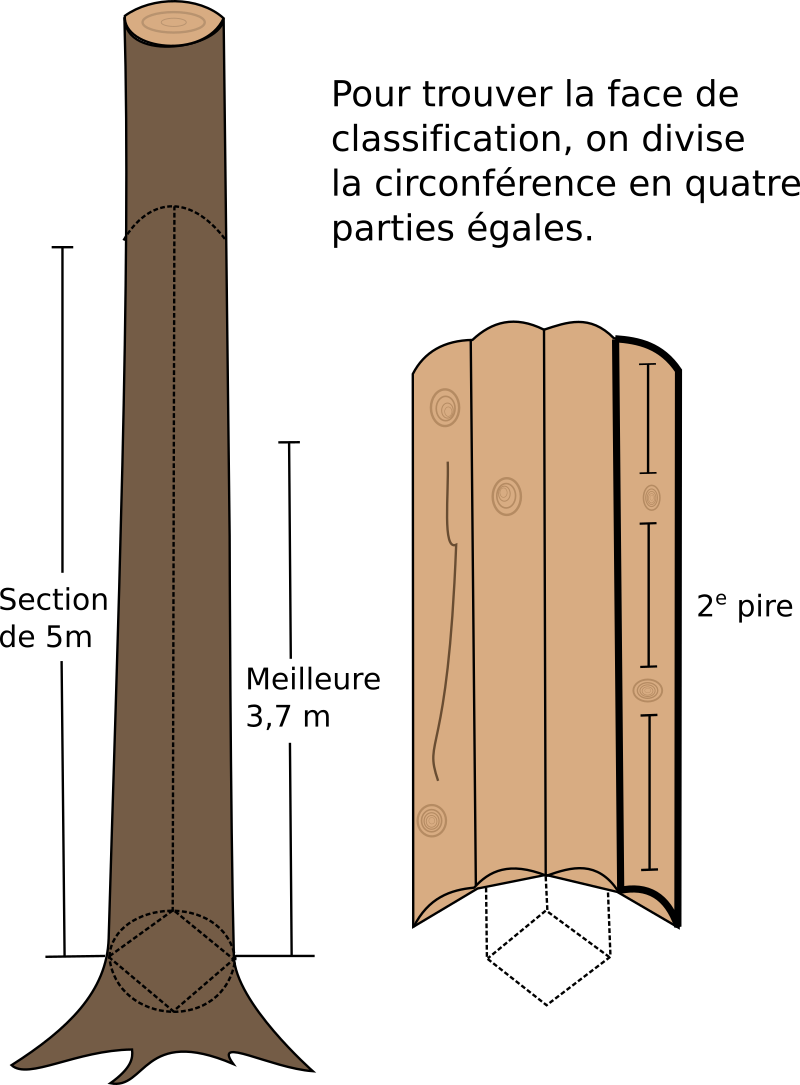
\includegraphics[width=0.5\linewidth]{img/ch8_Monger}
	\caption{Illustration du principe utilisé par le système de classification de la qualité des tiges d'essences feuillues. Le système est en vigueur au Québec depuis plusieurs décennies. Il permet d'estimer la valeur des bois sur pied, comme nous l'avons fait dans \cite{hassegawa2015large} \url{http://bit.ly/1gf2UNf}.}
	\label{fig:Monger}
\end{figure}

\subsection{La phase d'établissement du peuplement}

Lorsqu'on vise la régénération d'un peuplement forestier, on fait le choix entre la régénération naturelle ou le reboisement (plantation). Ces choix peuvent évidemment affecter la composition forestière (mélange d'espèces), ce qui aura éventuellement un impact sur les approvisionnements forestiers. Les choix qui sont effectués lors de cette phase n'auront toutefois qu'un impact à long terme sur les approvisionnements aux usines.

\subsubsection{La régénération naturelle}

La régénération naturelle est la méthode de régénération la plus opportuniste puisqu'on profite des éléments déjà en place. Ainsi, il est possible d'assurer la régénération du peuplement de façon économique. De plus, en utilisant l'ancien peuplement, on a plus de chances de régénérer des essences et des arbres mieux adaptés aux conditions de la station. Par contre, lorsque le capital sur pied est peu intéressant, il est possible que la régénération naturelle ne soit pas souhaitable. Au Québec, sur terres publiques, on a choisi de miser en priorité sur l'établissement d'une régénération naturelle.\\

\subsubsection{La régénération artificielle}

La régénération artificielle permet de remettre en production les superficies peu ou mal régénérées naturellement, soit 15 à 18\% des superficies exploitées au Québec \citep{thiffault2003sylviculture}. Grâce à l'utilisation d'espèces à croissance rapide ou de semences améliorées génétiquement, les plantations permettent d'augmenter le rendement des forêts. Ce rendement accru peut, en contrepartie, causer un déclin des propriétés du bois telles que la masse volumique chez les résineux, par exemple. Toutefois, les programmes de sélection génétique ont contribué à produire des plants à la fois hautement productifs et aux propriétés du bois désirables.\\

Après avoir choisi les plants à utiliser, le forestier doit déterminer la densité de reboisement. Les facteurs à prendre en compte sont alors la forme de la tige, la mortalité et la grosseur des branches, la qualité du bois, la production à l'hectare ainsi que par arbre, la survie, la stabilité de la plantation, la rentabilité des éclaircies et les aspects économiques. Cependant, presque toutes les études économiques ont convergé vers de très faibles valeurs de densité optimale \citep{thiffault2003sylviculture}. Au Québec, la densité préconisée (en forêt résineuse) est de 2000 tiges ha\up{-1}.\\

\subsection{Les travaux d'éducation des semis}

Le but premier du sylviculteur qui établit un nouveau peuplement forestier est d'assurer l'établissement d'un régénération libre de croître et occupant l'ensemble du site. Différents travaux peuvent être appliqués lorsque ces conditions ne sont pas réunies (Figure~\ref{fig:debrous}).\\

Pour combler les espaces inoccupés, deux actions sont possibles: le regarni et l'enrichissement. Le premier s'adresse aux peuplements reboisés ou ensemencés pour "garnir à nouveau". L'enrichissement permet d'introduire de nouvelles essences plus résistantes, plus performantes ou plus rentables. À titre d'exemple, c'est le cas lorsqu'on introduit de l'épinette blanche dans la régénération de sapin baumier ou encore du chêne rouge ou du pin blanc dans la régénération d'érable à sucre et de hêtre. Le dépressage est la simple action de réduire la densité. Cette opération est souvent faite systématiquement à ce stade. 


\begin{figure}[!h]
	\centering
	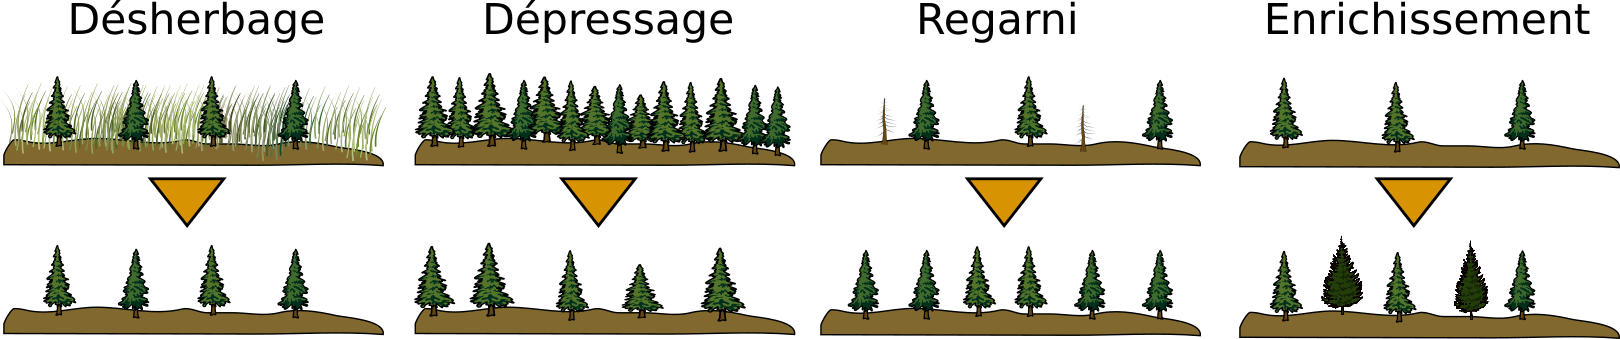
\includegraphics[width=1\linewidth]{./img/ch8_debrous}
	\caption{Différents travaux d'éducation au stade semis}
	\label{fig:debrous}
\end{figure}



\subsection{Les travaux précommerciaux}

Le nettoiement, le dépressage et le dégagement  au stade gaulis constituent trois types d'interventions que l'on regroupe au Québec dans la catégorie des « éclaircies précommerciales » (Figure \ref{fig:precom}). Elles sont très régulièrement appliquées au Québec. Elles ont deux impacts principaux sur la qualité future est approvisionnements: 1) elles permettent de contrôler la composition en espèces; 2) elles donnent plus de lumière aux arbres résiduels, ce qui leur permet de développer une cime plus vigoureuse.\\

\begin{figure}[!h]
	\centering
	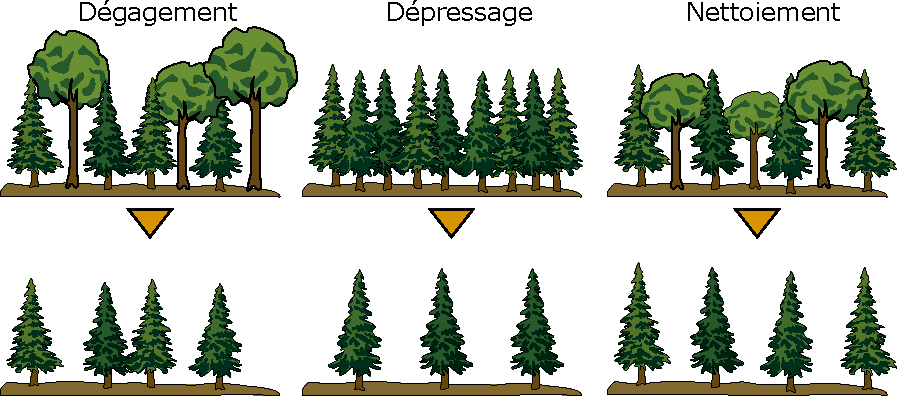
\includegraphics[width=1\linewidth]{./img/ch8_precom}
	\caption{Différents types d'éclaircies précommerciales au stade gaulis}
	\label{fig:precom}
\end{figure}

\subsection{Les travaux d'éclaircie commerciale}\label{ecomm}

L'éclaircie est dite « commerciale » lorsque les tiges coupées sont d'assez bonnes dimensions pour être transformées. Retenons deux systèmes d'éclaircies généralement reconnus dans la littérature : l'éclaircie par le bas et l'éclaircie par le haut.\\

\subsubsection{Éclaircie par le bas}

L'éclaircie par le bas consiste à retirer les tiges des classes intermédiaires et opprimées (voir figure \ref{fig:bas}). Elle permet de récupérer la mortalité imminente des tiges. Ainsi, l'approvisionnement associé à ce traitement sera surtout constitué de petites tiges peu vigoureuses et possiblement mal formées. Il s'agit d'un sacrifice à faire dans l'immédiat pour l'amélioration de la qualité et de la taille des tiges du peuplement lors de la coupe finale.\\ 

\begin{figure}[!h]
	\centering
	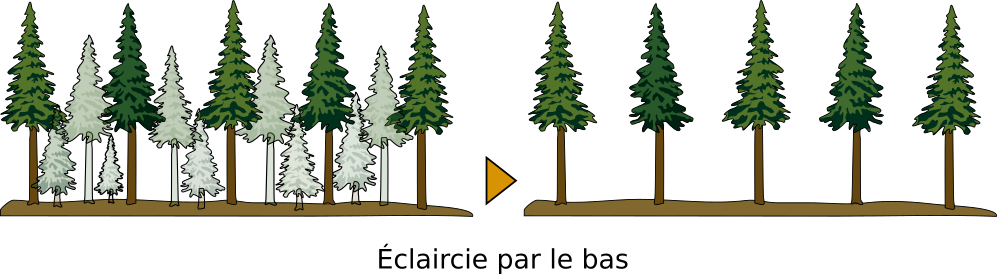
\includegraphics[width=1\linewidth]{./img/ch8_bas}
	\caption{Éclaircie par le bas}
	\label{fig:bas}
\end{figure}

\subsubsection{Éclaircie par le haut}

L'éclaircie par le haut consiste à éliminer un nombre déterminé de tiges des étages supérieurs afin de diminuer la densité du peuplement et de favoriser le développement des tiges d'avenir. Cette technique d'éclaircie est particulièrement utile pour stimuler le plus possible la croissance des tiges d'avenir \citep{smith1997practice} (voir Figure \ref{fig:haut}).\\

L'éclaircie par le haut diffère de l'éclaircie par le bas de deux façons : 1) elle s'applique à l'étage supérieur et 2) les tiges opprimées et intermédiaires qui ne gênent pas les tiges d'avenir demeurent en tout temps conservées dans le peuplement. Le fait de conserver l'étage inférieur possède plusieurs avantages dont celui d'éduquer les tiges d'avenir. La présence de voisins limite le développement de grosses branches (qui formeront de gros nœuds) dans les étages inférieurs.

\begin{figure}[!h]
	\centering
	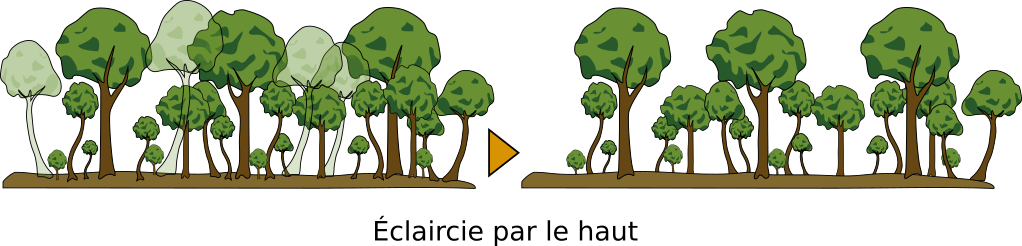
\includegraphics[width=1\linewidth]{./img/ch8_haut}
	\caption{Éclaircie par le haut}
	\label{fig:haut}
\end{figure}


\subsection{Choix du moment d'éclaircie}

Plusieurs moyens, à la fois qualitatifs ou quantitatifs, peuvent être utilisés pour déterminer le moment d'éclaircir. Le pourcentage de cime vivante est souvent utilisé comme indice. Si le pourcentage de cime vivante se situe entre la demie et le cinquième de la longueur des arbres, il est temps d'effectuer l'éclaircie. S'il dépasse la demie, il est trop tôt puisque le pourcentage élevé de cime vivante indique que l'accès à la lumière ne représente pas un facteur limitant la croissance radiale. À l'inverse, s'il est plus faible que le cinquième, il est trop tard puisque la capacité de l'arbre à réagir à l'ouverture du couvert est fortement diminuée (figure \ref{fig:cime}). Dans un tel cas l'arbre aurait à redévelopper son appareil photosynthétique, ce qui peut prendre plusieurs années.\\

\begin{figure}[!h]
	\centering
	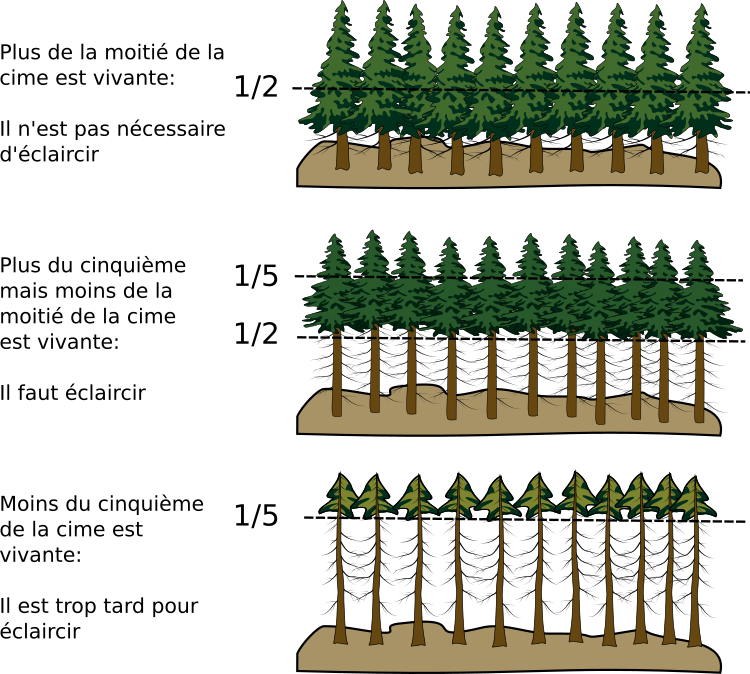
\includegraphics[width=0.8\linewidth]{./img/ch8_cime}
	\caption{Choix du moment d'éclaircie}
	\label{fig:cime}
\end{figure}

\subsection{La sylviculture en un clin d'œil}

Outre le choix des espèces à régénérer et faire croître, le principal outil de la sylviculture est le contrôle de la lumière apporté à l'arbre par la modification de l'espacement. Comme nous l'avons vu à la section~\ref{section_auxines}, c'est la lumière disponible qui contrôle le développement de la cime de l'arbre. Plus l'arbre reçoit de lumière, plus il développera une cime vigoureuse, ce qui accélérera la croissance radiale en raison de la disponibilité des produits de la photosynthèse et de la concentration élevée des auxines qui stimulent l'activité cambiale.

Les sylviculteurs visent à obtenir un espacement permettant d'occuper entièrement le territoire (production optimale en volume de bois rond par hectare) tout en favorisant une croissance radiale élevée. Toutefois, comme nous avons commencé à le voir dans les chapitres précédents, une croissance radiale élevée peut être accompagnée de diminutions des propriétés physico-mécaniques, comme la masse volumique chez les résineux, par exemple. L'identification d'un espacement optimal entre les arbres est donc très complexe, d'autant plus qu'on ignore souvent l'usage auquel sera destiné le bois produit. L'échelle du temps est donc importante à considérer lorsqu'on désire évaluer l'impact des traitements sylvicoles sur les propriétés des approvisionnements en bois. Les choix effectués dans le contexte:

\begin{description}
	\item[de la plantation] n'auront une influence que sur les approvisionnements dans un futur lointain. Dans nos conditions, à part quelques plantations à croissance rapide (peupliers et mélèzes hybrides), on peut considérer que la récolte ne s'effectuera pas avant 40 ans. Quelle seront les demandes du marché à ce moment? Il s'agit d'une question à laquelle il est à toutes fins pratiques impossible de répondre.
	\item[des soins aux semis,] de la même manière que pour la plantation, n'auront une influence que sur les approvisionnements dans un futur lointain.
	\item[des travaux précommerciaux] n'auront une influence que sur les approvisionnements dans un futur lointain. La définition des travaux précommerciaux implique que les arbres coupés soient laissés en forêt. On applique ces traitements aux peuplement de 10 à 20 ans. Il y a donc toujours une longue échéance entre l'application du traitement et la récolte finale.
	\item[des éclaircies commerciales et des coupes d'ensemencement] auront à la fois des conséquences sur les caractéristiques des approvisionnements dans l'immédiat et dans un futur assez proche. Dans le premier cas, des arbres (souvent de qualité moindre) sont récoltés pour des fins commerciales. L'applicabilité de ces traitement dépend donc souvent de la disponibilité de voies de valorisation pour ces bois de moindre qualité. Dans le deuxième cas, on peut espérer obtenir lors de la coupe finale des tiges de bonnes dimensions d'essences et de caractéristiques désirables. La coupe finale s'effectue généralement dans un délai de 10 à 20 ans, donc il est moins ardu de prévoir la structure du marché à cette échéance. 
\end{description}

\section{Propriétés indicatrices de la qualité du bois}

\begin{description}
	\item[La masse volumique] n'est généralement pas une variable directement indicatrice de la qualité du bois. En effet, il est rare que ce soit la masse volumique elle-même qui détermine l'aptitude du bois pour un usage donné. On considère plutôt la masse volumique comme un indicateur \og universel \fg de la qualité du bois. Ce fait s'explique par la corrélation qu'on retrouve entre la masse volumique et plusieurs propriétés physico-mécaniques (rigidité, résistance mécanique, retrait, dureté, etc.).
	\item[L'angle des microfibrilles] de la paroi secondaire est un critère important de détermination de la qualité du bois. Premièrement, un angle des microfibrilles élevé est associé à une moins grande rigidité. De plus, tel qu’on l’a vu au chapitre~\ref{paroi}, un angle prononcé des microfibrilles dans la paroi S\sub{2} engendre un retrait longitudinal élevé. L'angle des microfibrilles est donc un facteur important à considérer pour des usages du bois en structure.
	\item[La longueur des fibres et des trachéides] est considérée comme étant importante pour l'industrie des pâtes et papiers puisque des fibres plus longues donnent un papier plus résistant. Aussi, comme elle est inversement proportionnelle à l'angle des microfibrilles, elle est corrélée à plusieurs propriétés physico-mécaniques.
	\item[L'orientation du fil] est un caractère important du point de vue de la production de bois de dimension. Idéalement, l’axe longitudinal des fibres doit être parallèle à celui de la pièce. Une orientation non parallèle occasionne d'importantes pertes de propriétés mécaniques en plus de causer des défauts de rabotage et du gauchissement au séchage. L'alignement est souvent déterminé par le patron de sciage des billes, mais il peut aussi être occasionné par des déviations du fil à l'intérieur de la tige. Chez certains arbres poussant dans des endroits où les vents sont importants, les fibres peuvent être disposées avec un angle important (jusqu’à 35\degre par rapport à l’axe de la tige). On parle alors de fil spiralé. 
	\item[Les nœuds] peuvent affecter à la fois les propriétés mécaniques et l'apparence du bois. Un nœud est la partie d'une branche englobée dans le bois à la suite de la croissance de celui-ci. Tant que la branche demeure vivante, son cambium est relié à celui de la tige et il en résulte un nœud \og adhérent \fg. Dans le cas d'une branche morte, la continuité du cambium est brisée et le nœud qui en résulte est non adhérent. Les nœuds constituent des défaut locaux où s'initie la rupture (le MOR peut s'en voir sévèrement affecté). Ainis, la présence des nœuds joue un rôle majeur dans la classification des bois, et donc dans leur valeur. Tel qu’illustré à la Figure~\ref{fig:noeuds}, plus les pièces sont de grandes dimensions, plus la taille admissible des nœuds augmente. De plus, plus les nœuds sont situés près des rives des pièces, plus ils doivent être petits pour une classe donnée. Le traitement \og d'élagage \fg consiste à couper les branches du bas de la cime près du tronc, ce qui fait que le bois produit par la suite à cette hauteur dans la tige sera dépourvu de nœuds. 
	\item[Les propriétés mécaniques] sont importantes pour plusieurs usages du bois. Dans le cas de résineux utilisé en structure, la rigidité (MOE) et la résistance en flexion (MOR) sont les deux propriétés les plus souvent évaluées. En Europe, les pièces de bois utilisées en construction doivent avoir fait l'objet d'un classement mécanique préalable. Le plus souvent, il s'agit d'une mesure du MOE effectuée directement sur la ligne de production. On attribue une classe de rigidité à chaque pièce de bois, ce qui permet d'estimer statistiquement le module de rupture de la population des pièces de la même classe. Les classes les plus élevées ont une plus grande valeur. Elles servent le plus souvent à la fabrication des poutres et solives. Des classes moins élevées sont utilisées dans les montants de murs à ossature en bois. Les pièces des grades trop faibles ne peuvent servir que pour d'autres usages, tels que les clôtures et galeries. En Amérique du Nord le système des bois classés mécaniquement (MSR: \textit{Machine-stress-rated}) existe aussi, mais il ne sert qu'à certaines composantes spécifiques pour lesquelles des propriétés mécaniques élevées sont requises. Au Québec, on estime la production de bois MSR à 5\% de la production totale dans le groupe SEPM. Chez les feuillus nobles, les propriétés en flexion sont moins importantes pour les usages les plus communs (lames de plancher et meubles). Dans ce cas, la dureté revêt en revanche une plus grande importance.
	\item[La stabilité dimensionnelle] est l'une des caractéristiques les plus importantes à prendre en compte dans l'usage du bois. Elle affecte un très grands nombre de produits finis. Il est à noter, que les changements dimensionnels du bois en fonction de sa teneur en humidité sont inévitables. On ne peut donc pas les éliminer. Il importe toutefois de noter quelques points importants. 1) Les retraits tangentiel et radial sont assez importants chez toutes les espèces. Le ratio entre les deux est  typiquement de 2:1, mais il est plus faible chez certaines espèces, ce qui les rend aptes à certains usages comme la fabrication de cadres et moulures. 2) Le retrait longitudinal est très faible dans le bois mature. Il s'agit d'une qualité importante du bois utilisé dans les montants et les poutres des bâtiments. Toutefois, le retrait longitudinal peut devenir \hyperref[gonflement]{beaucoup plus élevé} lorsque l'angle des microfibrilles de la paroi S\sub{2} augmente, comme c'est le cas dans le bois juvénile et dans le bois de réaction. 3) Des problèmes importants de gauchissement peuvent survenir lorsque l'angle des microfibrilles d'une même pièce de bois varie de façon marquée.
\end{description}

\begin{figure}[!h]
	\centering
	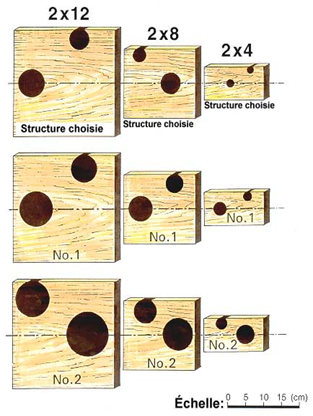
\includegraphics[width=0.5\linewidth]{./img/ch8_noeuds}
	\caption{Tailles maximales des nœuds permises sur les rives et au centre de pièces de 2$\times$4, 2$\times$8 et 2$\times$12 pour le groupe épinette-pin-sapin (adapté de \cite{jozsa1994discussion}}
	\label{fig:noeuds}
\end{figure}

\section{Le bois juvénile et le bois mature}

Le \textbf{bois juvénile} présente des caractéristiques indésirables pour plusieurs applications. Il est produit pendant les 10 à 30 premiers cernes  de croissance et se présente dans l'arbre comme une colonne partant de la souche et allant jusqu'au sommet de l'arbre tel qu'illustré à la Figure~\ref{fig:juv_aubier}. En fait, l'appellation \og bois juvénile \fg n'est qu'une catégorisation des courbes de tendance présentées au chapitre~\ref{variabilite}. En réalité, la zone juvénile est une zone dans laquelle les propriétés du bois évoluent rapidement depuis la moelle. La zone de bois mature correspond au contraire à l'endroit où les propriétés varient peu en fonction de l'âge cambial.\\

\begin{figure}[!h]
	\centering
	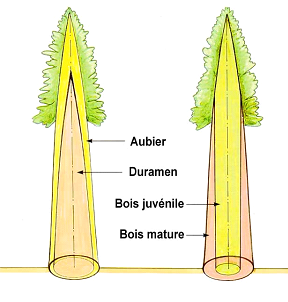
\includegraphics[width=0.5\linewidth]{./img/ch8_juv_aubier}
	\caption{Distribution du bois d’aubier et de duramen et du bois juvénile et mature (adapté de \cite{jozsa1994discussion})}
	\label{fig:juv_aubier}
\end{figure}

Les caractéristiques remarquables du bois juvénile sont les suivantes:

\begin{itemize}
	\item fibres plus courtes que celles du bois mature;
	\item angle des microfibrilles plus fort que celui du bois mature (Figure~\ref{fig:juv_comp});
	\item teneur en cellulose plus faible que celle du bois mature;
	\item plus forte proportion de nœuds que le bois mature, mais ceux-ci sont généralement adhérents (puisque produits par des branches vivantes);
	\item une masse volumique plus faible chez les bois de type I, mais plus élevée chez le type III (il n'y a pas de patron simple pour le type II). 
\end{itemize}

\begin{figure}[!h]
	\centering
	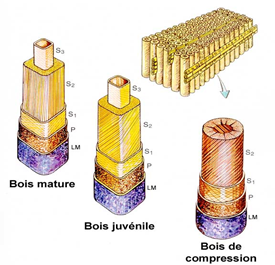
\includegraphics[width=0.5\linewidth]{./img/ch8_juv_comp}
	\caption{Orientation des microfibrilles dans le bois mature, le bois juvénile et le bois de compression (adapté de \cite{jozsa1994discussion})}
	\label{fig:juv_comp}
\end{figure}


Voici quelques raisons proposées permettant d'expliquer les avantages évolutifs de patron typique de variation des propriétés du bois (nommé PRT ci-après pour \og patron radial typique \fg) de la moelle vers l'écorce \citep{lachenbruch2011radial}.

\begin{description}
\item[L'hypothèse biomécanique] associe le PRT à une adaptation évolutive aux différents types de stimuli biomécaniques qu'un arbre doit subir au cours de sa vie. Elle présente l'arbre comme un bras de levier ayant un moment de résistance maximal au vent. Les jeunes pousses doivent résister à des stimuli mécaniques complexes provenant du vent. Afin de réduire le moment de force généré par l'action du vent, une bonne stratégie biomécanique consiste à fléchir de manière marquée, ce qui diminue la longueur du bras de levier par rapport à l'axe de rotation. Une telle stratégie demande à la fois une grande flexibilité (angle des microfibrilles élevé) et une contrainte maximale à la rupture élevée. Cette stratégie ne serait toutefois pas applicable dans une tige de plus forte dimension puisque la masse de l'arbre qui penche génère un moment de force supplémentaire. Le besoin grandissant de limiter la déformation de la tige engendrée par ces stimuli alors que la tige devient plus volumineuse expliquerait le PRT.

\item[L'hypothèse hydraulique] associe plutôt le PRT à la nécessité de maintenir une conductivité hydraulique efficace dans le xylème, et ce, tant chez les jeunes arbres de faibles dimensions que chez les arbres plus âgés beaucoup plus grands. Ainsi, les cellules formées près de la moelle étant de masse plus faible, et n'ayant accès qu'à un système racinaire peu développé chez les jeunes arbres, auraient un accès plus limité à des réserves d'eau. Elle devraient donc être plus flexibles afin de pouvoir résister à une pression négative élevée (causée par \hyperref[eau]{l'évapotranspiration}). Au contraire, les cellules du bois mature auraient avantage à être plus rigides tout en augmentant leur capacité de transport pour compenser les forces attribuables à la friction et la gravité dans des conduits beaucoup plus longs.

\item[L'hypothèse du développement] implique plutôt que le PRT résulte de l'évolution des propriétés des cellules cambiales. Ainsi, les propriétés seraient moins avantageuses dans le bois juvénile parce que le jeune cambium n'a tout simplement pas la capacité de produire du bois aux caractéristiques \og idéales \fg. Un exemple de cette théorie a été présenté \hyperref[prt_longueur]{pour expliquer l'évolution de la longueur des trachéides et des fibres de la moelle vers l'écorce}. Dans ce cas, il n'est pas possible que le cambium produise de longues fibres près de la moelle puisque le taux de cloisonnement anticlinal y est élevé et que celui-ci réduit la taille des initiales.\\
\end{description}

Il est fort probable que tous ces mécanismes entrent en jeu dans la détermination du PRT. En comprenant mieux les impacts de chacun des mécanismes, on arrivera à mieux contrôler les effets de nos choix sylvicoles sur la qualité du bois.\\

La présence du bois juvénile a plusieurs impacts sur les propriétés du bois. En plus des caractéristiques mentionnées précédemment, on note :

\begin{itemize}
\item Le retrait longitudinal jusqu'à cinq fois supérieur du bois juvénile par rapport au bois mature qui augmente les risques de gauchissement;
\item La rigidité inférieure du bois juvénile par rapport à celle du bois mature;
\item Le rendement plus faible du bois juvénile pour la production de pâte et de papier par rapport à celle du bois mature.
\item Le module d'élasticité (MOE) de sciages contenant 100\% de bois juvénile peut être de 50 à 60\% inférieur à celui de sciages qui n'en contiennent pas.
\end{itemize}

Le bois juvénile a donc certaines similitudes avec le \hyperref[compression]{bois de compression} qui se développe chez les espèces résineuses sous l'effet d'une pente, des vents dominants ou de cimes déséquilibrées. La présence de bois de compression réduit aussi la résistance mécanique et augmente le retrait longitudinal à cause de l'angle des microfibrilles très fort. La forme des cellules est toutefois bien différente, tel qu’illustré à la Figure~\ref{fig:juv_comp}.

Il importe aussi de distinguer la distribution caractéristique du bois de duramen et d'aubier de celle du bois juvénile (Figure~\ref{fig:juv_aubier}). La proportion de bois de duramen revêt peut être reliée à la qualité du bois, en particulier pour les usages où une bonne résistance à la pourriture et aux insectes est requise (thuya occidental, genévrier) et ceux où la couleur du bois est importante (noyer noir, cerisier tardif). Comme il a déjà été mentionné, le bois de duramen est plus résistant à la pourriture et aux insectes que le bois d'aubier à cause des extractibles qu'il contient, mais il est également moins perméable que le bois d'aubier.
 

\section{Effets de la sylviculture sur la distribution des propriétés du bois dans la tige}

Jusqu'à présent dans ce cours, la variation des propriétés du bois vous a été présentée à plusieurs échelles, soit entre les cellules d'un même cerne, entre les cernes d'un même arbre et entre les espèces. La sylviculture implique la choix des espèces à régénérer et faire croître, \hyperref[tab:grostab]{ce qui influencera en retour les propriétés du bois produit}.\\

Au-delà du choix des espèces, la sylviculture peut avoir une grande influence sur les propriétés du bois de par la modification du patron radial de croissance, et donc de la distribution des propriétés du bois dans la tige. La proportion de bois juvénile à l'échelle de l'ensemble de la tige dépend:

\begin{enumerate}
	\item de l'âge de l'arbre;
	\item de la vigueur et du développement de la cime;
	\item du patron de croissance dans le temps. 
\end{enumerate}
	
Chacune de ces variables peuvent être contrôlées par la sylviculture. La proportion de bois juvénile dans un arbre est fonction du taux de croissance dans les premières années de de développement de l'arbre. À diamètre égal, un arbre à croissance rapide contiendra plus de bois juvénile qu'un arbre à croissance lente n'ayant pas une cime très développée. En corollaire à cela, des mesures prises pour accélérer la croissance en bas âge peuvent faire augmenter la proportion de bois juvénile et même prolonger la période de production de bois juvénile. L'espacement initial, suivi du régimes d'éclaircies pouvant être appliquées ont donc une forte influence sur la distribution des propriétés du bois dans les tiges des arbres.\\ 
	
\subsection{La théorie de Larson}

Revenons sur la \hyperref[section_auxines]{théorie de Larson} pour bien comprendre les effets de l'espacement initial et du régime des éclaircies sur les propriétés du bois. Cette théorie relie le patron radial typique de variation des propriétés du bois, soit l'une des sources de variation les plus importantes, à la production d'auxines dans la cime vivante \citep{larson1969wood}. Lorsque le cambium est situé à proximité d'une cime vigoureuse bénéficiant d'un bon apport en lumière du soleil, la concentration d'hormones de croissance est élevée. Une concentration élevée d'auxines stimule une croissance rapide, ce qui entraînera la production de bois aux caractéristiques juvéniles (trachéides et fibres plus courtes, angle de microfibrilles de la paroi S\sub{2} plus prononcé, etc.), et ainsi de propriétés mécaniques plus faibles.\\

Ici, il importe de comprendre que même dans un arbre placé toute sa vie en pleine lumière, il y aura tout de même une évolution progressive des propriétés du bois de la moelle à l'écorce. L'allongement des branches et l'ombre que se font les branches entre elles font en sort qu'il y aura nécessairement un éloignement progressif de cette source d'auxines engendrant ainsi l'amélioration graduelle des propriétés du bois. Donc, retenons les principes suivants. Par le contrôle de l'espacement entre les arbres:

\begin{itemize}
	\item \textbf{La sylviculture peut avoir léger impact sur la durée de la production de bois aux caractéristiques juvénile}. Ce prolongement s'expliquerait par le fait qu'à un âge cambial donné, un cerne situé à proximité d'une cime vigoureuse aura tendance à avoir des propriétés légèrement moindres par rapport à un cerne appartenant à un arbre dont la cime est plus petite. Ce fait est illustré par un exemple à la Figure~\ref{fig:auty_mfa}.
	\item \textbf{La sylviculture a une influence importante sur la taille de la zone juvénile dans une tige}. Dans l'exemple de la Figure~\ref{fig:auty_mfa}, les 10 premiers cernes de croissance tendent à produire du bois avec un angle de microfibrilles particulièrement élevés, et ce, peu importe la vigueur de la cime. Ainsi, l'impact le plus important de la vigueur de la cime sera d'influence l'espace occupé par les 10 premier cernes de croissance dans une tige donnée.
\end{itemize}

\begin{figure}[ht]
	\centering
	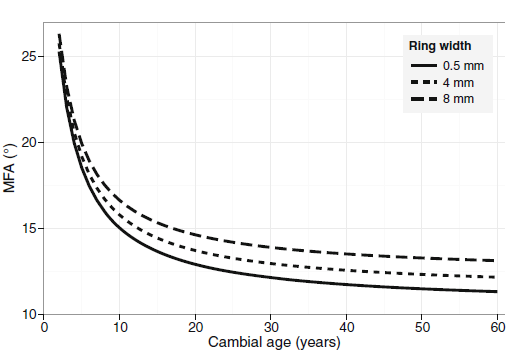
\includegraphics[width=0.8\linewidth]{img/ch8_auty_mfa}
	\caption{Illustration de l'importance du patron de variation de la moelle vers l'écorce par rapport à la vigueur de la cime chez le pin sylvestre (\textit{Pinus sylvestris}). Le patron de variation pour le scénario de croissance radiale le plus rapide (lui-même associé à une cime vigoureuse) se place légèrement sous les deux autres. MFA représente l'angle des microfibrilles de la paroi S\sub{2}. Image tirée de \cite{auty2013models}}
	\label{fig:auty_mfa}
\end{figure}

\subsection{{Des exemples idéalisés de scénarios sylvicoles}}

Pour illustrer les principes évoqués à la section précédente, imaginons d'abord un scénario sylvicole menant à la production de bois de faible qualité. Ce scénario comprendrait:
\begin{itemize}
	\item un espacement initial large entre les arbres;
	\item une augmentation progressive de l'espacement par des éclaircies répétées;
	\item une coupe finale en bas âge puisque les arbres auront atteint des dimensions commerciales très tôt.
\end{itemize}

Un tel scénario engendrerait une forte proportion de bois juvénile dans les tiges. Afin de limiter les conséquences néfastes d'un tel scénario sylvicole sur les propriétés du bois, on peut avoir recours à la sélection génétique des meilleurs sujets pour la plantation et à l'élagage progressif des tiges du bas de la cime. Il s'agit d'un choix d'approche sylvicole communément appliqué dans les plantation de pin radiata (\textit{Pinus radiata}) en Nouvelle-Zélande et au Chili, par exemple.\\

Imaginons maintenant un scénario sylvicole à l'inverse, axé sur la production de bois aux propriétés physico-mécaniques élevées. Ce scénario comprendrait:

\begin{itemize}
	\item un espacement initial étroit entre les arbres, tel qu'obtenu par l'établissement d'une régénération naturelle dense;
	\item une augmentation progressive de l'espacement par des éclaircies répétées, mais tardives, qui auront l'avantage de stimuler la croissance radiale alors que l'arbre produit du bois mature (au bas de la tige);
	\item une coupe finale à un âge avancé, ce qui augmentera la proportion de bois mature.
\end{itemize}

Il s'agit d'un choix d'approche sylvicole plus souvent appliqué dans des pays comme la Suisse, l'Allemagne et la France. Il mène à la production de bois de qualité, mais sur de très longues révolutions.\\

\subsection{Scénario sylvicole typiquement appliqué au Québec}

Les arbres de groupe SEPM constituent la grande majorité des bois récoltés au Québec et, encore aujourd'hui, la grande majorité des bois récoltés provient de peuplements naturels non aménagés. Ceux-ci tirent le plus souvent leur origine d'une régénération naturelle installée à la suite de perturbations naturelles (feux, épidémies d'insectes, chablis). Comme leur croissance radiale était généralement lente et que les arbres sont récoltés à un âge élevé, les propriétés physico-mécaniques des ces bois sont généralement élevées. Toutefois, à mesure que la récolte progresse vers le nord, la taille des arbres tend à diminuer, ce qui limite la productivité des opérations de récolte et de transformation. Pour tirer notre épingle du jeu à l'échelle internationale, nous sommes ainsi \og forcés \fg de miser sur des solutions technologiques axées sur une production à valeur ajoutée.\\

Malgré ce fait, on applique maintenant depuis plusieurs années au Québec une sylviculture qui commencera bientôt à porter ses fruits. De manière générale, pour le groupe SEPM, on peut considérer que notre sylviculture ne déviera pas dans une large mesure de la situation actuelle, c'est-à-dire qu'elle mise sur la production à long terme de bois de qualité relativement élevée. Typiquement, nos scénarios sylvicoles comprennent:

\begin{itemize}
	\item un espacement initial étroit entre les arbres, puisqu'on mise surtout sur la régénération naturelle dense (la plantation ne touche que 20\% des territoires remis en production annuellement);
	\item une augmentation de l'espacement entre les arbres par le biais d'éclaircies commerciales pratiquées lorsque le peuplement atteint l'âge de 10 à 15 ans;
	\item une coupe finale qui sera effectuée lorsque les arbres auront un âge avancé, ce qui augmentera la proportion de bois mature.
\end{itemize} 

Le scénario sylvicole présenté ici résume toutefois assez bien l'approche qui a été mise de l'avant dans les peuplements qui arriveront à maturité lors des prochaines décennies. Malgré les traitements d'éclaircie précommerciale, il y a fort à parier que les faibles dimensions des tiges demeureront un facteur limitant la productivité des usines de transformation des bois du groupe SEPM, mais nous devrions en contrepartie continuer de miser sur un bois aux propriétés physico-mécanique élevées.\\

Il existe bien sûr une grande variété de scénarios sylvicoles appliqués sur notre vaste territoire et ceux-ci produiront des résultats fort variables. Il n'existe d'ailleurs pas de réponse simple que l'on puisse donner à la question: quel sera l'impact d'un scénario sylvicole sur les propriétés du bois? Il existe une infinité de scénarios possibles, que l'on peut appliquer à un grand nombre d'espèces sur une multitude de stations. Voilà pourquoi une approche de modélisation est généralement privilégiée.